\documentclass[aspectratio=169,10pt]{beamer}

\usetheme{Madrid}
\usecolortheme{seahorse}
\usepackage{amsmath,amssymb,amsfonts}
\usepackage{mathtools}
\usepackage{listings}
\usepackage{xcolor}
\usepackage{graphicx}
\usepackage{hyperref}
\usepackage{array}
\usepackage{calc}
\usepackage{tikz}

% Graphics path
\graphicspath{{figures/}}

% Beamer customization
\setbeamertemplate{footline}[frame number]
\setbeamertemplate{navigation symbols}{}

% Code listing style
\lstset{
    language=Python,
    basicstyle=\ttfamily\scriptsize,
    keywordstyle=\color{blue},
    commentstyle=\color{green!50!black}\itshape,
    stringstyle=\color{red},
    breaklines=true,
    frame=single,
    numbers=left,
    numbersep=5pt,
    showstringspaces=false,
    tabsize=2
}

% Custom colors
\definecolor{darkblue}{HTML}{1f77b4}
\definecolor{darkred}{HTML}{d62728}
\definecolor{darkgreen}{HTML}{2ca02c}

\title{Chapter 9c: Applications of Fixed Point Theorems}
\subtitle{Integral and Integrodifferential Equations}
\author{Pathak's Nonlinear Analysis}
\date{\today}

% ============================================================================
% PRESENTATION BEGINS
% ============================================================================
\begin{document}

\frame{\titlepage}

% ============================================================================
% SECTION: Overview
% ============================================================================
\section{Overview}

\begin{frame}{Chapter 9: Applications of Fixed Point Theorems}
\begin{itemize}
    \item<1-> \textbf{9.1}: Existence of solutions to differential equations
    \item<2-> \textbf{9.2}: Existence of solutions to differential inclusions
    \item<3-> \textbf{9.3}: Common solutions via operator splitting
    \item<4-> \textbf{9.4}: Applications to periodic problems
    \item<5-> \textbf{9.5}: \textcolor{darkred}{Applications to nonlinear integral equations}
    \item<6-> \textbf{9.6}: \textcolor{darkblue}{Applications to abstract Volterra integrodifferential equations}
\end{itemize}

\vspace{2em}
\visible<7->{
\textbf{Focus of this chapter:}
\begin{itemize}
    \item Existence and uniqueness theorems for integral equations
    \item Fixed point methods and contraction mappings
    \item Cone methods for positivity preservation
    \item Integrodifferential equations with operator semigroups
\end{itemize}
}
\end{frame}

\begin{frame}{Key Concepts and Tools}
\begin{columns}[T]
\column{0.5\textwidth}
\textbf{Integral Equations:}
\begin{itemize}
    \item Volterra equations
    \item Fredholm equations
    \item Urysohn operators
    \item Generalizations
\end{itemize}

\vspace{1em}
\textbf{Fixed Point Methods:}
\begin{itemize}
    \item Contraction mappings
    \item Darbo's theorem
    \item Measure of noncompactness
\end{itemize}

\column{0.5\textwidth}
\textbf{Functional Spaces:}
\begin{itemize}
    \item $C[a,b]$ (continuous functions)
    \item $L_p$ spaces
    \item Cone structures
\end{itemize}

\vspace{1em}
\textbf{Operators:}
\begin{itemize}
    \item Integral operators
    \item $C_0$-semigroups
    \item Infinitesimal generators
\end{itemize}
\end{columns}
\end{frame}

% ============================================================================
% SECTION: Section 9.5 - Nonlinear Integral Equations
% ============================================================================
\section{9.5: Nonlinear Integral Equations}

\begin{frame}{Volterra Integral Equations}
\begin{definition}
A \textbf{Volterra integral equation} of the second kind is:
\[
x(t) = \lambda \int_a^t f(t, s, x(s))ds + y(t), \quad t \in [a,b]
\]
where $\lambda$ is a parameter, $f$ is a given function, and $y$ is the inhomogeneous term.
\end{definition}

\vspace{1em}
\visible<2->{
\begin{theorem}[Classical Contraction Solution]
If $|f(t,s,\xi) - f(t,s,\eta)| \leq F(t,s)|\xi - \eta|$ with
\[
k = \sup_{t \in [a,b]} \left\{ \int_a^t F(t,s)ds \right\} < 1
\]
then the Volterra equation has a unique solution in $C[a,b]$.
\end{theorem}
}

\visible<3->{
\textbf{Key observation:} The contraction factor improves with the integral, making convergence fast.
}
\end{frame}

\begin{frame}{Urysohn Operator}
\begin{definition}
The \textbf{Urysohn operator} is defined by:
\[
[Ux](t) = \int_\Omega f(t, s, x(s))ds
\]
where integration is over a domain $\Omega$.
\end{definition}

\vspace{1em}
\visible<2->{
\begin{theorem}[Positivity in Cones]
Let $X = C[a,b]$, and $K$ be the cone of nonnegative functions. If:
\begin{enumerate}
    \item $U$ maps $K$ into itself
    \item $U$ is continuous and maps bounded sets into precompact sets
    \item Suitable boundary conditions hold
\end{enumerate}
then the equation $Ux = x$ has a positive solution.
\end{theorem}
}

\visible<3->{
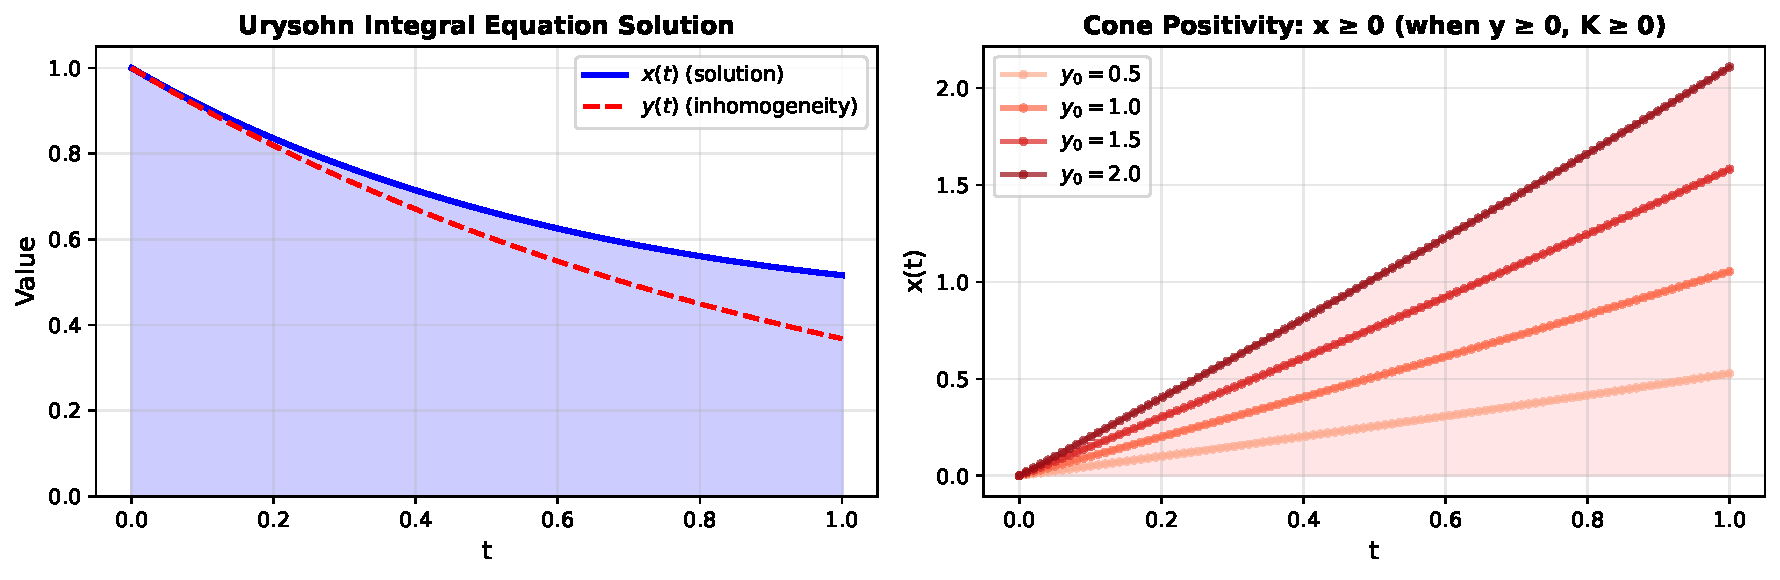
\includegraphics[width=0.6\textwidth]{urysohn_operator}
}
\end{frame}

\begin{frame}[fragile]{Theorem 9.26: Himmelberg's Lemma Application}
\begin{theorem}
Let $X$ be a separable reflexive Banach space and $C \subset X$ a closed convex subset.
Suppose $\varphi_x: X \to Y$ is a continuous map for each $x \in C$ such that:
\begin{enumerate}
    \item $(x_n \to x$ in $C, $u_n \to u$ in $X) \Rightarrow \varphi_{x_n}(u_n) \to \varphi_x(u)$
    \item The set $C_x = \{u \in X : \varphi_x(u) = 0\}$ is nonempty, closed, and convex
    \item $C_x \cap B_r \neq \emptyset$ for each $x \in C$
\end{enumerate}
then $\varphi_x(x) = 0$ has a solution in $C$.
\end{theorem}

\vspace{1em}
\textbf{Application to Integral Equations:} Setting $\varphi_x(u) = u - Ux$ where $U$ is
an integral operator, we obtain solutions to nonlinear integral equations.
\end{frame}

\begin{frame}[fragile]{Theorem 9.27: Nonlinear Integral Equations}
\begin{theorem}
Consider the integral equation:
\[
x(s) = y(s) + \int_0^1 K(s,t)x(t)dt, \quad s \in [0,1]
\]
Suppose:
\begin{enumerate}
    \item $K(s,t) \geq 0$ a.e. on $[0,1] \times [0,1]$
    \item $\text{ess}\sup_{t \in [0,1]} \int_0^1 K^2(s,t)dt < \infty$
    \item $y(s) \geq 0$ a.e. on $[0,1]$
\end{enumerate}
Then the equation has a solution $x \in L_2[0,1]$ with $0 \leq x(s) \leq y(s)$ a.e.
\end{theorem}

\vspace{1em}
\visible<2->{
\textbf{Key idea:} Using cone positivity and Himmelberg's lemma, we guarantee
positive solutions under mild conditions on kernels.
}
\end{frame}

\begin{frame}{Theorem 9.30: Periodic Solutions}
\begin{theorem}
Consider the nonlinear integral equation:
\[
x(t) = q(t) + \int_0^\beta f(t,s,x(\phi(s)))ds + \int_0^{\sigma(t)} g(t,s,x(\phi(s)))ds
\]
Suppose certain conditions hold on $f$, $g$, and the domain $[0,\beta]$. Then the equation
has a positive $p$-periodic solution defined on $\mathbb{R}$.
\end{theorem}

\vspace{1em}
\visible<2->{

\includegraphics[width=0.8\textwidth]{fixed_point_iteration}
}
\end{frame}

\begin{frame}[fragile]{Theorem 9.32: Darbo Condition for Integral Operators}
\begin{theorem}
Assume $\Omega \subset C[a,b]$ is nonempty, bounded, convex, and closed. Let $P$ and $T$
map $\Omega$ continuously into itself with $P(\Omega)$ and $T(\Omega)$ bounded.
If $P$ and $T$ satisfy the Darbo condition with constants $k_1, k_2$:
\[
\|P(\Omega)\|_k_2 + \|T(\Omega)\|_{k_1} < 1
\]
then $S = P \circ T$ is a contraction with respect to the measure of noncompactness
$\omega$ with constant $\|P(\Omega)\|_{k_2} + \|T(\Omega)\|_{k_1}$,
and has at least one fixed point in $\Omega$.
\end{theorem}

\vspace{1em}
\visible<2->{
\textbf{Advantage over Banach:} Darbo's theorem applies to non-contractive operators
via the Hausdorff measure of noncompactness.
}
\end{frame}

% ============================================================================
% EXAMPLES AND APPLICATIONS
% ============================================================================
\section{Examples and Applications}

\begin{frame}[fragile]{Example: Generalized Nonlinear Functional-Integral Equations}
Consider the generalized nonlinear functional-integral equation (GNFIE):
\[
x(t) = f\left(t,x(\theta(t)), \int_0^{\beta(t)} f(t,s,x(\phi(s)))ds,
        \int_0^{\sigma(t)} g(t,s,x(\phi(s)))ds\right)
\]

\vspace{1em}
\textbf{Special cases:}

\begin{tabular}{|l|l|}
\hline
\textbf{When} & \textbf{Reduces to} \\
\hline
$\sigma(t) = \infty$, $g = 0$ & Nonlinear Fredholm IE (9.124) \\
$\sigma(t) = \infty$, $F(t,x) = f$ & Integral equation (9.125) \\
$F(t,x) = f(t,x_2, x_4)$ & Nonlinear IE (9.126) \\
$F = p(t,x_1) + x_2 x_4$ & Quadratic integral IE (9.127) \\
$F = x_1 + p(x_3,x_4)$ & Functional-integral IE (9.131) \\
\hline
\end{tabular}

\vspace{1em}
\visible<2->{
Each case can be studied separately with appropriate fixed point theorems!
}
\end{frame}

\begin{frame}{Special Cases of Integral Equations}
\begin{enumerate}
    \item \textbf{Volterra IE (9.144):} $x(t) = a(t) + \int_0^t p(t,s,x(s))ds$

    \item \textbf{Urysohn IE (9.145):} $x(t) = b(t) + \int_0^a q(t,s,x(s))ds$

    \item \textbf{Functional IE (9.146):} $x(t) = a(t)\int_0^a q(t,s,x(s))ds + \left(\int_0^t p(t,s,x(s))ds\right)\left(\int_0^a q(t,s,x(s))ds\right)$

    \item \textbf{Chandrasekhar IE (9.147):} $x(t) = 1 + x(t)\int_0^a \frac{t}{t+s}\varphi(s)x(s)ds$
\end{enumerate}

\vspace{1.5em}
\visible<2->{
\textbf{Common theme:} All can be analyzed using fixed point theory via
contraction properties or cone methods!
}
\end{frame}

\begin{frame}[fragile]{Numerical Example: Volterra Integral Equation}
\begin{lstlisting}
# Solve: x(t) = sin(t) + 0.3*integral_0^t (t-s)*x(s) ds

import numpy as np
from scipy.integrate import odeint

def volterra_kernel(t, s):
    """Volterra kernel K(t,s) = t - s"""
    return max(t - s, 0)

def solve_volterra(kernel, y, t, iterations=5):
    """Fixed point iteration for Volterra equation"""
    x = y.copy()
    for k in range(iterations):
        x_new = np.zeros_like(x)
        for i, t_i in enumerate(t):
            # Numerical integration
            integral = 0
            for j in range(i):
                integral += 0.3 * kernel(t_i, t[j]) * x[j]
            x_new[i] = y[i] + integral
        x = x_new
    return x

# Parameters
t = np.linspace(0, 1, 100)
y = np.sin(t)
x_solution = solve_volterra(volterra_kernel, y, t)
\end{lstlisting}
\end{frame}

\begin{frame}{Visualization of Volterra Kernel}
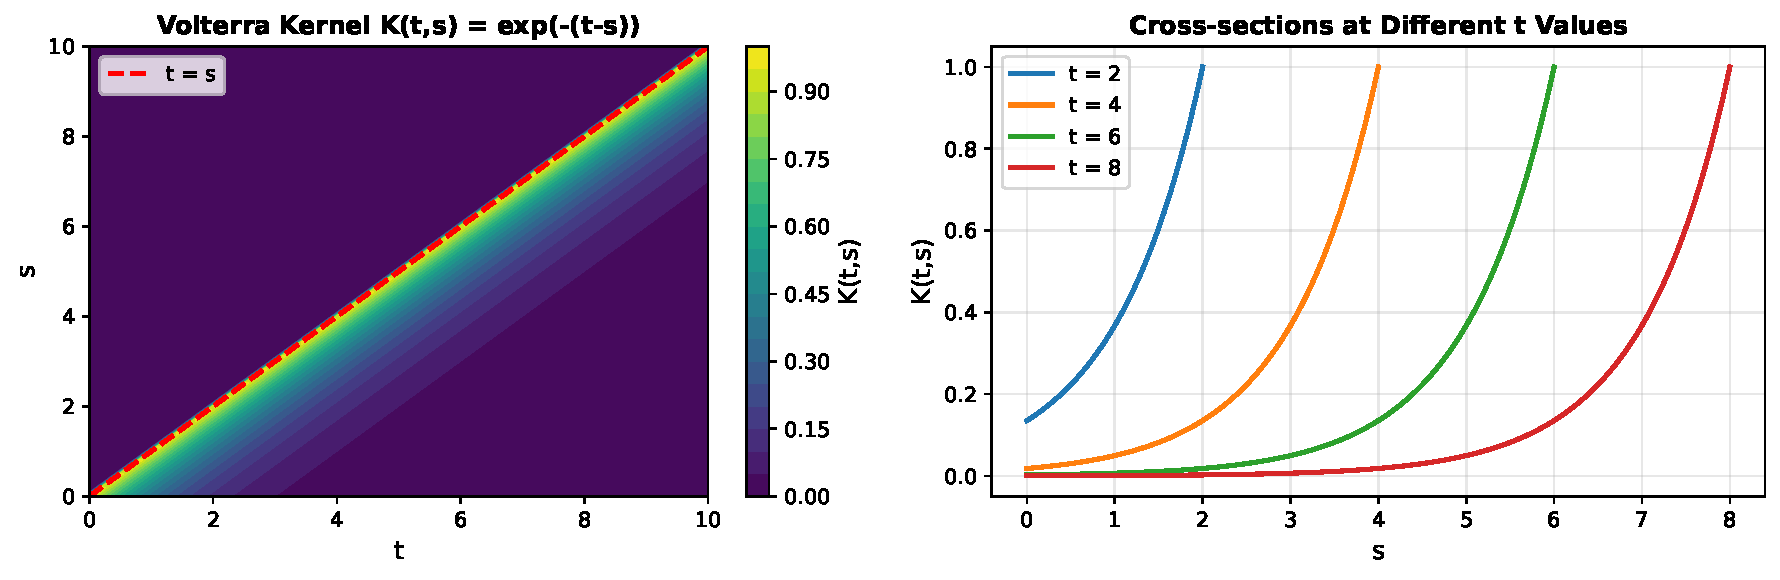
\includegraphics[width=\textwidth]{volterra_kernel}

The left plot shows the Volterra kernel $K(t,s) = e^{-(t-s)}$ as a contourf,
while the right shows cross-sections at different $t$ values. The causal structure
$K(t,s) = 0$ for $t < s$ is essential for existence of solutions.
\end{frame}

% ============================================================================
% SECTION 9.6 - INTEGRODIFFERENTIAL EQUATIONS
% ============================================================================
\section{9.6: Integrodifferential Equations}

\begin{frame}{Abstract Volterra Integrodifferential Equations}
\begin{definition}
An abstract Volterra integrodifferential equation of the form:
\[
u'(t) + Au(t) = f(t,u(t)) + \int_{t_0}^t g\left(t,s,u(s),\int_{t_0}^s K_1(s,\tau,u(\tau))d\tau\right)ds
\]
where:
\begin{itemize}
    \item $-A$ is the infinitesimal generator of a $C_0$-semigroup $\{T(t)\}_{t \geq 0}$
    \item $f, g$ are given continuous functions
    \item $K_1, K_2$ are integral kernels
\end{itemize}
\end{definition}

\vspace{1em}
\visible<2->{
\textbf{Mild solution:} A continuous $u(t)$ is a mild solution if:
\[
u(t) = T(t-t_0)u_0 + \int_{t_0}^t T(t-s)f(s,u(s))ds + \int_{t_0}^t T(t-s)\mathcal{K}(s)ds
\]
where $\mathcal{K}(s)$ denotes the integral term.
}
\end{frame}

\begin{frame}{Key Assumptions for IDEs}
\textbf{Hypothesis $(H_1)$:} Functions $u, f, g$ are continuous and bounded on relevant domains.

\vspace{0.8em}
\textbf{Hypothesis $(H_2)$:} Lipschitz conditions:
\begin{align}
|u(t,x_1) - u(t,x_2)| &\leq a_1(t)|x_1 - x_2| \\
|f(t,y_1,x_1) - f(t,y_2,x_2)| &\leq a_2(t)|y_1 - y_2| + a_3(t)|x_1 - x_2| \\
|g(t,y_1,x_1) - g(t,y_2,x_2)| &\leq a_4(t)|y_1 - y_2| + a_5(t)|x_1 - x_2|
\end{align}

\vspace{0.8em}
\textbf{Hypothesis $(H_3)$:} Continuous functions form the set $\mathcal{C} = [0,a] \times [0,a]$
mapping into $[0,a] \times \mathbb{R}$.

\vspace{0.8em}
\textbf{Hypothesis $(H_4)$:} $\max\{a_1, a_2, a_3, a_4, a_5\}(t) \leq k$ (boundedness).

\vspace{0.8em}
\textbf{Hypothesis $(H_6)$:} $4\gamma \eta < 1$ where $\gamma = k + ka\beta$,
$\eta = kaa\ell + m$ (contraction condition).
\end{frame}

\begin{frame}{Theorem 9.34: Common Mild Solution}
\begin{theorem}
Consider the equations:
\begin{align}
u'(t) + Au(t) &= f(t,u(t)) + \int_{t_0}^t g\left(t,s,u(s),\int_{t_0}^s K_1(s,\tau,u(\tau))d\tau\right)ds \\
u'(t) + Au(t) &= \bar{f}(t,u(t)) + \int_{t_0}^t \bar{g}\left(t,s,u(s),\int_{t_0}^s \bar{K}_1(s,\tau,u(\tau))d\tau\right)ds
\end{align}

Under hypotheses $(H_1)$-$(H_6)$, these equations have a common mild solution in $B_r$.
\end{theorem}

\vspace{1em}
\visible<2->{
\textbf{Proof technique:} Define operators $T_1, T_2$ for each equation and use
fixed point iteration on their composition.
}
\end{frame}

\begin{frame}[fragile]{Integrodifferential Equation Solution}
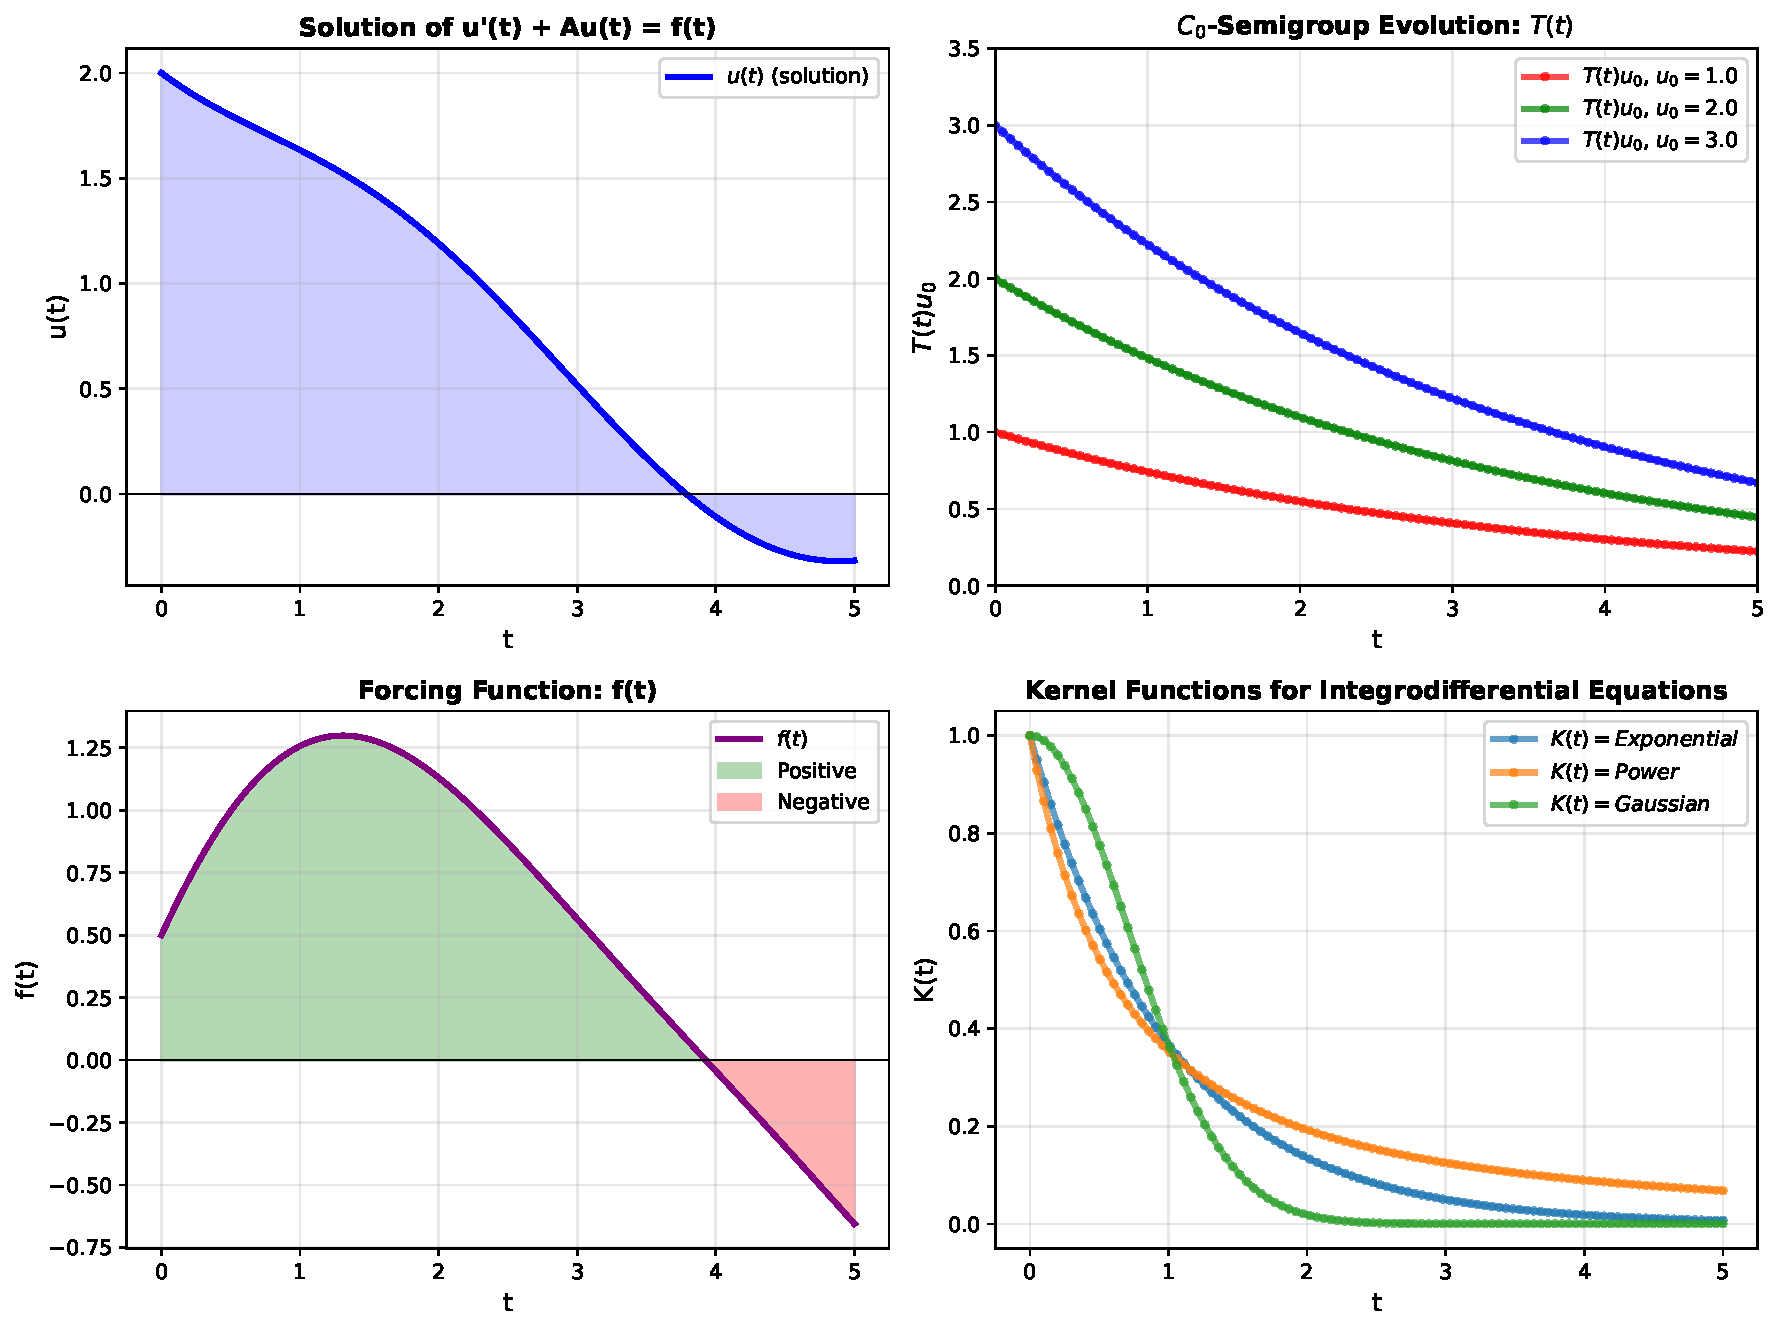
\includegraphics[width=\textwidth]{integrodifferential}

Top-left: Solution trajectory. Top-right: $C_0$-semigroup evolution.
Bottom-left: Forcing function $f(t)$. Bottom-right: Different kernel types.
\end{frame}

% ============================================================================
% CONVERGENCE AND STABILITY
% ============================================================================
\section{Convergence and Stability}

\begin{frame}{Convergence Results}
\begin{theorem}[Rates of Convergence]
For the contraction operator $U$ with contraction constant $k < 1$,
the iterates $U^n x_0$ converge to the fixed point $x^*$ with:
\[
\|U^n x_0 - x^*\| \leq \frac{k^n}{1-k}\|Ux_0 - x_0\|
\]

The convergence is:
\begin{enumerate}
    \item \textbf{Linear} if $k$ is constant
    \item \textbf{Superlinear} if $k$ depends on iteration and $k_n \to 0$
    \item \textbf{Quadratic} if $k_n = O(\|U^n x_0 - x^*\|)$
\end{enumerate}
\end{theorem}

\vspace{1em}
\visible<2->{
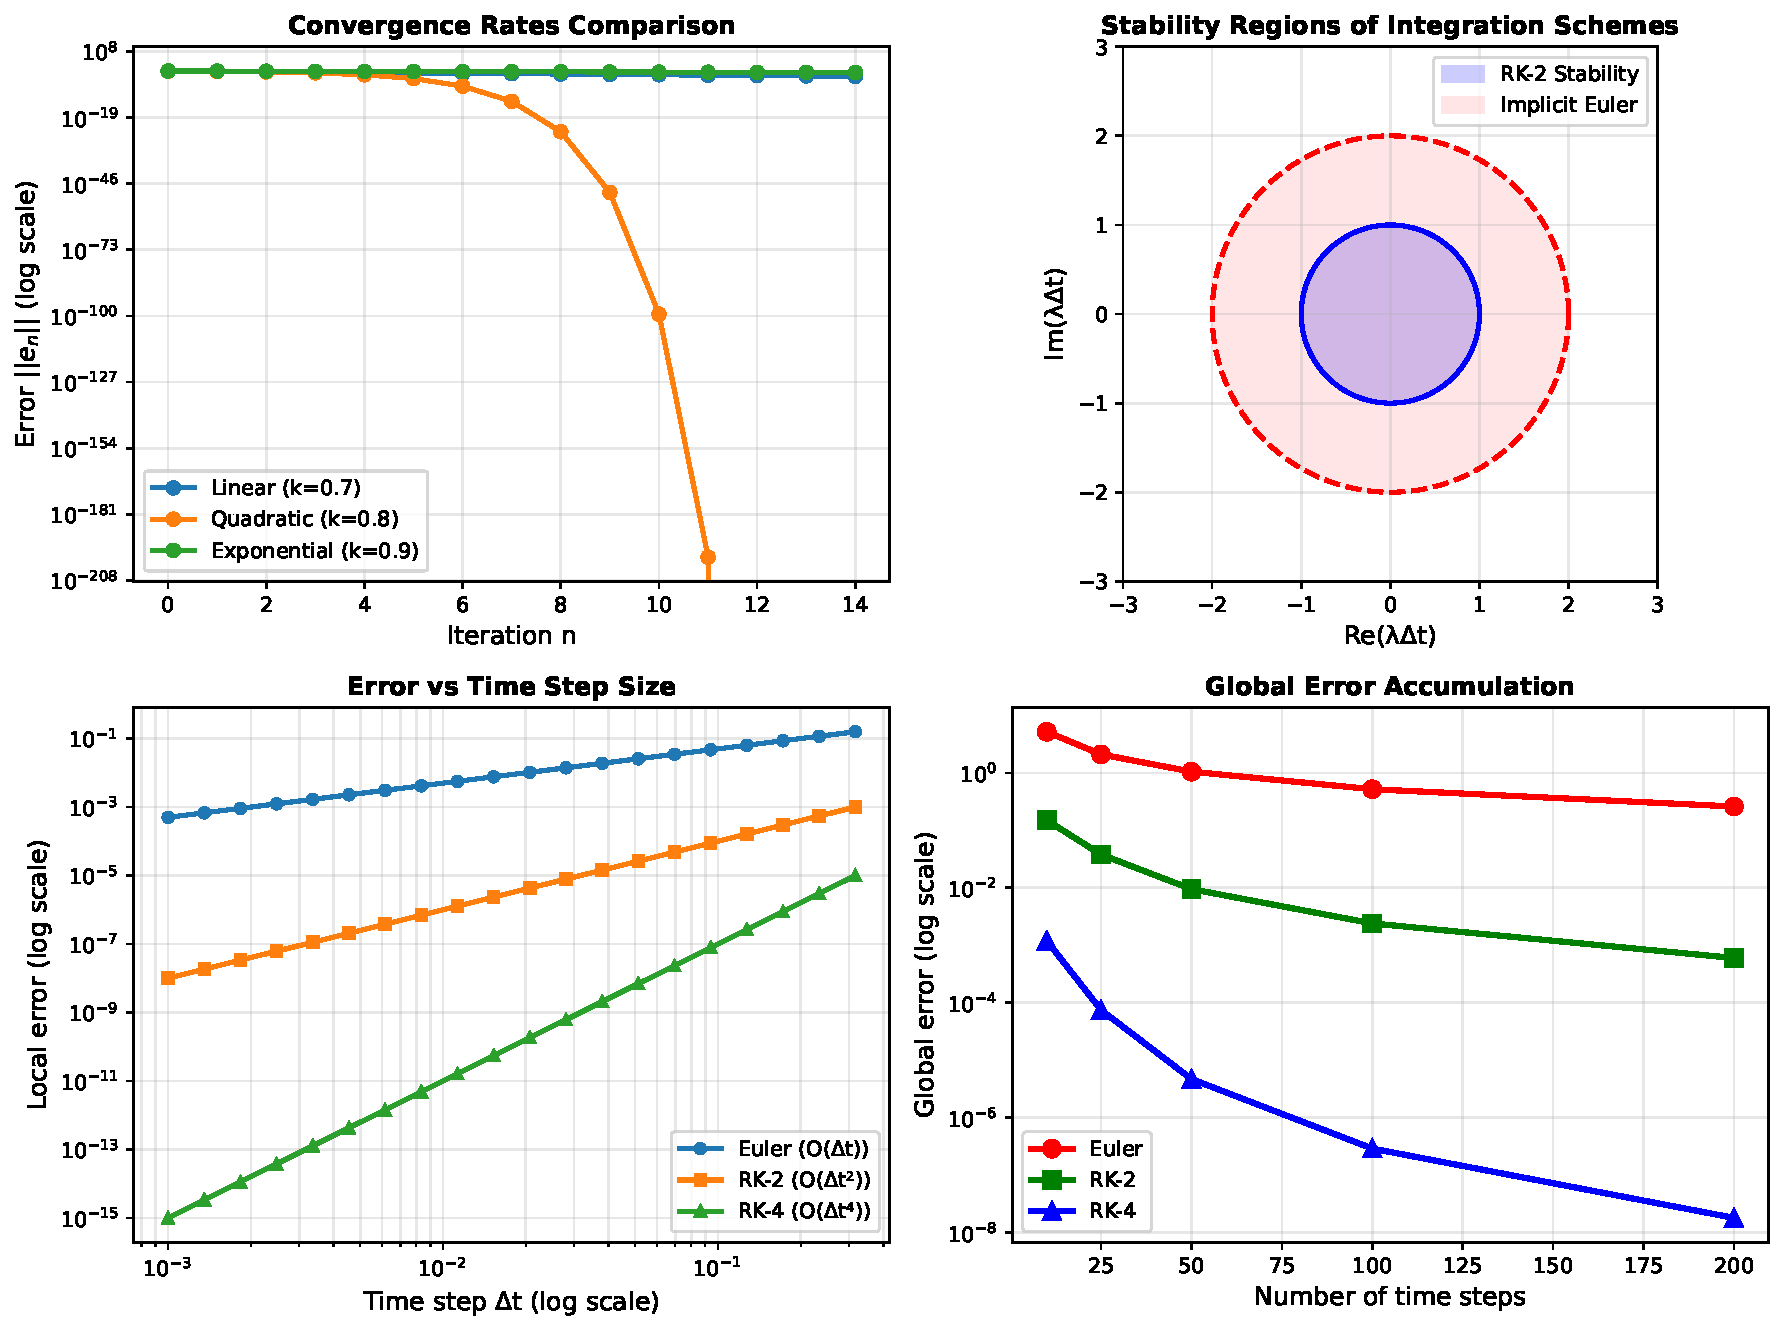
\includegraphics[width=0.7\textwidth]{convergence_stability}
}
\end{frame}

\begin{frame}{Stability Analysis}
\begin{theorem}[Stability of Solutions]
If $U$ is a contraction mapping on a Banach space $X$, then:
\begin{enumerate}
    \item The unique fixed point $x^*$ is \textbf{globally asymptotically stable}
    \item Small perturbations in initial data lead to small perturbations in solutions
    \item The solution depends continuously on parameters
\end{enumerate}
\end{theorem}

\vspace{1em}
\textbf{For numerical schemes:} The stability depends on the step size $\Delta t$:

\begin{itemize}
    \item \textbf{Explicit Euler}: Stable if $\lambda \Delta t$ lies in unit disk
    \item \textbf{Implicit Euler}: Stable for all $\Delta t > 0$ (unconditionally stable)
    \item \textbf{RK-4}: Stable for $|\lambda \Delta t| \leq 2.78$ (larger region)
\end{itemize}
\end{frame}

% ============================================================================
% DARBO'S THEOREM AND MEASURE OF NONCOMPACTNESS
% ============================================================================
\section{Darbo's Theorem}

\begin{frame}{Measure of Noncompactness}
\begin{definition}
The \textbf{Hausdorff measure of noncompactness} $\omega(A)$ of a bounded set $A$ is:
\[
\omega(A) = \inf\{d > 0 : A \text{ can be covered by finitely many sets of diameter} \leq d\}
\]
\end{definition}

\vspace{1em}
\textbf{Properties:}
\begin{enumerate}
    \item $\omega(A) = 0$ iff $A$ is compact (or precompact)
    \item $\omega(A) = \omega(\overline{A}) = \omega(\text{conv}(A))$
    \item $\omega(A \cup B) = \max\{\omega(A), \omega(B)\}$
    \item $\omega(A + B) \leq \omega(A) + \omega(B)$
\end{enumerate}

\vspace{1em}
\visible<2->{
\textbf{Key insight:} Measures of noncompactness generalize compactness to infinite-dimensional spaces.
}
\end{frame}

\begin{frame}{Darbo's Fixed Point Theorem}
\begin{theorem}[Darbo, 1955]
Let $K$ be a nonempty, bounded, convex, and closed subset of a Banach space $X$,
and let $T: K \to K$ be a continuous operator. If there exists a constant $k \in [0,1)$
such that:
\[
\omega(T(A)) \leq k \cdot \omega(A)
\]
for all bounded subsets $A \subseteq K$, then $T$ has at least one fixed point in $K$.
\end{theorem}

\vspace{1em}
\visible<2->{
\textbf{Advantages:}
\begin{itemize}
    \item Applies to operators that are \textbf{not contractive} in classical sense
    \item Works in spaces without metrics (only seminorms)
    \item Extends Banach fixed point theorem substantially
\end{itemize}
}
\end{frame}

\begin{frame}{Darbo Condition Visualization}

\includegraphics[width=\textwidth]{darbo_condition}

Top-left: Function satisfying Lipschitz condition. Top-right: Darbo contraction of measure.
Bottom-left: Decay of measure of noncompactness. Bottom-right: Comparison with Banach.
\end{frame}

% ============================================================================
% SUMMARY AND CONCLUSIONS
% ============================================================================
\section{Summary and Conclusions}

\begin{frame}{Main Results Summary}
\begin{enumerate}
    \item \textbf{Section 9.5:} Integral equations via fixed points
    \begin{itemize}
        \item Volterra equations with contraction constant $k < 1$
        \item Cone methods for positivity preservation
        \item Generalized functional-integral equations
        \item Multiple special cases (Fredholm, Urysohn, quadratic, etc.)
    \end{itemize}

    \vspace{1em}
    \item \textbf{Section 9.6:} Integrodifferential equations
    \begin{itemize}
        \item Abstract equations with infinitesimal generators
        \item $C_0$-semigroups and mild solutions
        \item Common solutions to pairs of equations
        \item Continuous dependence on data
    \end{itemize}
\end{enumerate}

\vspace{1em}
\visible<2->{
\textbf{Unifying theme:} Fixed point theory provides a powerful framework for
proving existence and uniqueness of solutions to complex integral and integrodifferential equations.
}
\end{frame}

\begin{frame}{Key Techniques}
\begin{columns}[T]
\column{0.5\textwidth}
\textbf{Functional Analysis:}
\begin{itemize}
    \item Banach spaces and norms
    \item Compactness and precompactness
    \item Measure of noncompactness
    \item Semigroup theory
\end{itemize}

\column{0.5\textwidth}
\textbf{Fixed Point Methods:}
\begin{itemize}
    \item Contraction mappings
    \item Darbo's theorem
    \item Himmelberg's lemma
    \item Krasnoselskii's theorem
\end{itemize}
\end{columns}

\vspace{2em}
\textbf{Application Strategy:}
\begin{enumerate}
    \item Formulate the problem as $Tx = x$ for an appropriate operator $T$
    \item Verify that $T$ maps a suitable set into itself
    \item Show $T$ is continuous and maps bounded sets appropriately
    \item Apply the relevant fixed point theorem
\end{enumerate}
\end{frame}

\begin{frame}[fragile]{Implementation Considerations}
\textbf{When solving integral equations numerically:}

\begin{enumerate}
    \item \textbf{Discretization:} Use quadrature rules (Simpson, trapezoidal)
    \begin{itemize}
        \item Higher order rules for smoother kernels
        \item Special care near singularities
    \end{itemize}

    \item \textbf{Iteration:} Fixed point iteration usually stable
    \begin{itemize}
        \item Gauss-Seidel faster than Jacobi
        \item Damping helps: $x_{n+1} = \alpha Tx_n + (1-\alpha)x_n$
    \end{itemize}

    \item \textbf{Stopping criterion:} Use error estimates
    \begin{itemize}
        \item A posteriori: $\|x_{n+1} - x_n\| < \epsilon$
        \item Or check: $\|Tx_n - x_n\| < \epsilon(1-k)$
    \end{itemize}
\end{enumerate}

\vspace{1em}
\textbf{For integrodifferential equations:} Use ODE solvers with semigroup evaluations.
\end{frame}

\begin{frame}{Open Problems and Extensions}
\begin{itemize}
    \item \textbf{Nonlinear growth:} $|f(t,s,\xi)| \leq a(t,s) + b(t,s)|\xi|^p$

    \item \textbf{Delay arguments:} $x(t) = \int_0^t f(t,s,x(\theta(s)))ds$

    \item \textbf{Fractional equations:} $D^\alpha x = f(t,x) + \int_0^t (t-s)^\beta x(s)ds$

    \item \textbf{Coupled systems:} Multiple equations with coupling terms

    \item \textbf{Singular kernels:} $K(t,s) = (t-s)^\alpha$ with $\alpha < 0$

    \item \textbf{Random equations:} Stochastic integral equations with noise
\end{itemize}

\vspace{1.5em}
\visible<2->{
\textbf{All extensions use similar fixed point methodology!}
}
\end{frame}

\begin{frame}[fragile]{References and Further Reading}
\begin{itemize}
    \item \textbf{Pathak, H. K.} (2018). \textit{An Introduction to Nonlinear Analysis and Fixed Point Theory}

    \item \textbf{Gripenberg, G., Londen, S. O., \& Staffans, O.} (1990). \textit{Volterra Integral and Functional Equations}

    \item \textbf{Krasnoselskii, M. A.} (1964). \textit{Topological Methods in the Theory of Nonlinear Integral Equations}

    \item \textbf{Kirk, W. A. \& Sims, B.} (2001). \textit{Handbook of Metric Fixed Point Theory}

    \item \textbf{Darbo, G.} (1955). ``Punti uniti in trasformazioni a condominio non compatto''

    \item \textbf{Himmelberg, C. J.} (1975). Fixed point theorems for compact multifunctions
\end{itemize}
\end{frame}

\begin{frame}[plain]
\begin{center}
\Huge \textbf{Thank You}

\vspace{2em}

\Large Chapter 9c: Applications of Fixed Point Theorems to \\
Integral and Integrodifferential Equations

\vspace{2em}

\normalsize For more information, see:
\textit{An Introduction to Nonlinear Analysis and Fixed Point Theory} (Pathak, 2018)
\end{center}
\end{frame}

\end{document}
